% Copyright 2016 by Wang Kunzhen <wangkunzhen1993@gmail.com>.
% Modified for Final Report Presentation

\documentclass[xcolor=dvipsnames]{beamer}

% Theme and Color Settings
\usetheme{Malmoe}

\definecolor{nus-orange}{RGB}{239,124,0} 
\definecolor{nus-white}{RGB}{255,255,255}
\definecolor{nus-blue}{RGB}{0,61,124}
\definecolor{nus-black}{RGB}{0,0,0}

\setbeamercolor{section in head/foot}{bg=nus-blue, fg=nus-white}
\setbeamercolor{subsection in head/foot}{bg=nus-blue, fg=nus-white}
\setbeamercolor{frametitle}{bg=nus-orange, fg=nus-black}
\setbeamercolor{title}{bg=nus-orange, fg=nus-white}
\setbeamercolor{alerted text}{fg=nus-orange}
\setbeamercolor{block title}{fg=nus-blue}
\setbeamercolor{block body}{fg=nus-black}

\setbeamertemplate{theorems}[numbered]
\setbeamertemplate{propositions}[numbered]
\setbeamertemplate{bibliography item}{\insertbiblabel}
\setbeamertemplate{title page}[default][colsep=-4bp,rounded=true, shadow=true]
\setbeamertemplate{navigation symbols}{} % Remove navigation symbols
\setbeamertemplate{footline}[frame number] % Add page numbers

\usepackage{booktabs}
\usepackage{graphicx}
\usepackage{amsmath}
\usepackage{colortbl}

% Metadata
\title{Final Report}
\subtitle{Application of Supervised Learning Methods to Transformation Mechanisms in DBPs Formation}
\author[Zhou Dafu]{Zhou Dafu \\ \small Supervisor: Prof. Hu Jiangyong}
\institute[NUS]
{
  Department of Civil and Environmental Engineering\\
  National University of Singapore
}
\titlegraphic{
   
\includegraphics[width=2cm]{nus-logo.png}
}
\date{May 7, 2026}

\begin{document}

% Title Slide
\begin{frame}
  \titlepage
\end{frame}

% Outline
\begin{frame}{Outline}
  \tableofcontents
\end{frame}

% ============================================================================
% Section 1: Introduction & Objectives
% ============================================================================
\section{Introduction \& Objectives}

\subsection{Background}
\begin{frame}{Background \& DBP Formation}
  \begin{block}{The Challenge}
    \begin{itemize}
        \item \textbf{Disinfection By-products (DBPs)}: Formed by the reaction of disinfectants (e.g., Chlorine) with Natural Organic Matter (NOM).
        \item \textbf{Health Concerns}: Potential carcinogenic properties (e.g., THMs, HAAs, Nitrosamines).
        \item \textbf{Goal}: Leverage high-frequency sensor data (TRC, pH, TOC) and Machine Learning for real-time predictive control.
    \end{itemize}
  \end{block}

  \begin{block}{Chemistry in Alkaline Conditions}
    \begin{itemize}
        \item $ \text{NH}_3 + \text{OCl}^- \rightarrow \text{NH}_2\text{Cl} + \text{OH}^- $
        \item Chloramines react with organic nitrogen precursors (secondary amines) leading to N-DBPs formation.
    \end{itemize}
  \end{block}
\end{frame}

\begin{frame}{Limitations of Traditional Approaches}
  \begin{block}{Methodological Gaps}
    \begin{itemize}
        \item \textbf{Complex Kinetics}: Mechanistic models struggle with non-linear, dynamic hydraulic conditions.
        \item \textbf{Infrequent Sampling}: Lab testing provides low temporal resolution and high costs.
    \end{itemize}
  \end{block}
  \begin{block}{The Deep Learning Opportunity}
    \begin{itemize}
        \item Capable of capturing intricate temporal dependencies from multi-variate continuous time-series data without explicit manual feature shifting.
    \end{itemize}
  \end{block}
\end{frame}

\subsection{Concepts}
\begin{frame}{Transfer Learning \& Fine-Tuning}
  \begin{block}{The Need for Transferability}
      \begin{itemize}
          \item Water sources and environmental conditions (e.g., temperature) vary significantly.
          \item Training entirely new models for every condition is computationally expensive and data-hungry.
      \end{itemize}
  \end{block}
  \begin{block}{Fine-Tuning Strategy}
      \begin{itemize}
          \item \textbf{Full Fine-Tuning}: Updating all weights on the new target dataset.
          \item \textbf{Partial Fine-Tuning (Frozen Encoder)}: Freezing feature extraction layers, updating only the predictive heads.
          \item \textbf{Adapter (LoRA)}: Injecting small trainable bottleneck layers to maintain parameter efficiency.
      \end{itemize}
  \end{block}
\end{frame}

\subsection{Objectives}
\begin{frame}{Objectives}
  \begin{block}{Core Research Goals}
    \begin{enumerate}
        \item \textbf{Evaluate Predictive Models}: Compare GBDTs (XGBoost, LightGBM, CatBoost) against Classical NNs (MLP, RNN, LSTM, GRU) and Modern Sequence Architectures (Transformer, Mamba).
        \item \textbf{Investigate Fine-Tuning}: Test the Transformer's capability to transfer learned kinetics across different temperatures ($29^{\circ}\text{C}$ to $35^{\circ}\text{C}$) and water sources (CAWW, LSWW).
        \item \textbf{Develop a Production GUI}: Package the machine learning backend into a user-friendly frontend application for facility operators.
    \end{enumerate}
  \end{block}
\end{frame}

% ============================================================================
% Section 2: Methodology
% ============================================================================
\section{Methodology \& Experimental Framework}

\subsection{System \& Data}
\begin{frame}{System Description}
  \begin{figure}
      \centering
      \includegraphics[width=0.8\textwidth]{../attachment/reactors.png}
      \caption{Simulated WDS: Disinfection (DT), Retention (RT), and Pipelines (PPL1/2).}
  \end{figure}
\end{frame}

\begin{frame}{Data Preprocessing: Stochastic Imputation}
  \begin{block}{Challenge \& Solution}
      \begin{itemize}
          \item Addresses 30-min alternating sensor gaps between PPL1 and PPL2.
          \item Fills gaps via linear regression combined with variance-matched random noise.
      \end{itemize}
  \end{block}
  \vspace{0.2cm}
  \begin{figure}
      \centering
      \includegraphics[width=0.6\textwidth,height=0.4\textheight,keepaspectratio]{../attachment/imputation.png}
  \end{figure}
\end{frame}

\begin{frame}{Data Preprocessing: Data Segmentation}
  \begin{block}{Sliding Window Approach}
      \begin{itemize}
          \item Instead of manual time-alignment, a sliding window implicitly captures hydraulic delay.
          \item \textbf{Split Ratio}: Chronological division of $7:1.5:1.5$ for Training, Validation, and Testing.
      \end{itemize}
  \end{block}
\end{frame}

\subsection{Models \& Strategies}
\begin{frame}{Model Architectures Overview}
  \begin{block}{GBDTs (Single-Output Regressors)}
      \begin{itemize}
          \item \textbf{XGBoost, LightGBM, CatBoost}: Fast, tree-based ensemble learners relying on histogram optimizations and regularization.
      \end{itemize}
  \end{block}
  \begin{block}{Neural Networks (Multi-Output Regressors)}
      \begin{itemize}
          \item \textbf{MLP}: Flattened baseline.
          \item \textbf{RNN, LSTM, GRU}: Recursive state updates capturing sequential logic.
          \item \textbf{Transformer}: Multi-head global self-attention.
          \item \textbf{Mamba}: State Space Model (SSM) enabling linear-time sequence processing.
      \end{itemize}
  \end{block}
\end{frame}

\begin{frame}{Transformer for Time Series: Why Encoder-Only?}
  \begin{block}{Attention over Time}
      \begin{itemize}
          \item Calculates attention weights across the entire sequence simultaneously.
          \item Captures global temporal dependencies and long-range correlations irrespective of distance.
      \end{itemize}
  \end{block}
  \begin{block}{Encoder-Only Rationale}
      \begin{itemize}
          \item \textbf{NLP vs Regression}: NLP translation requires a Decoder for auto-regressive generation of variable-length text.
          \item \textbf{Our Task}: Maps a fixed-length historical multi-variate input to concurrent numerical predictions.
          \item \textbf{Benefit}: Omitting the Decoder reduces overfitting and boosts computational efficiency while retaining feature extraction power.
      \end{itemize}
  \end{block}
\end{frame}

\subsection{Training Workflow}
\begin{frame}{Model Training Configuration}
  \begin{block}{Parameters}
    \begin{itemize}
        \item \textbf{Loss \& Optimization}: Mean Squared Error (MSE); Adam Optimizer for NNs.
        \item \textbf{Hyperparameters}: Tuned via Bayesian Optimization on the CAWW\_29 dataset.
    \end{itemize}
  \end{block}
\end{frame}

\begin{frame}{Model Training Workflow}
  \begin{figure}
      \centering
      \includegraphics[width=\textwidth,height=0.75\textheight,keepaspectratio]{../attachment/model workflow.png}
  \end{figure}
\end{frame}

\begin{frame}{Fine-Tuning Workflow}
  \begin{figure}
      \centering
      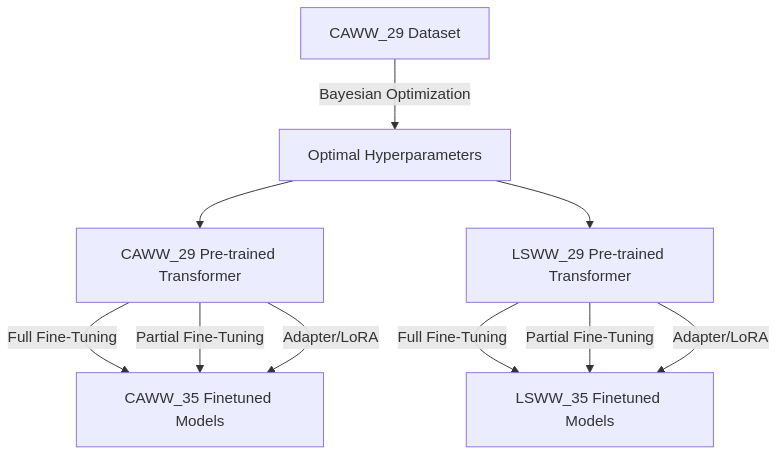
\includegraphics[width=0.75\textwidth]{../attachment/finetuning_workflow.png}
      \caption{Transferring knowledge from $29^{\circ}\text{C}$ baselines to $35^{\circ}\text{C}$ datasets.}
  \end{figure}
\end{frame}

% ============================================================================
% Section 3: GUI Development
% ============================================================================
\section{GUI Development}
\subsection{Software Tech Stack}
\begin{frame}{Frontend Software Application}
  \begin{columns}
      \begin{column}{0.5\textwidth}
          \begin{block}{Architecture}
              \begin{itemize}
                  \item \textbf{Vite}: Blazing fast build tool and HMR.
                  \item \textbf{React}: Component-based UI framework for state-driven interactions.
                  \item \textbf{Electron}: Packages the web app into a native desktop executable, granting local filesystem access to the Python backend.
              \end{itemize}
          \end{block}
      \end{column}
      \begin{column}{0.5\textwidth}
          \centering
          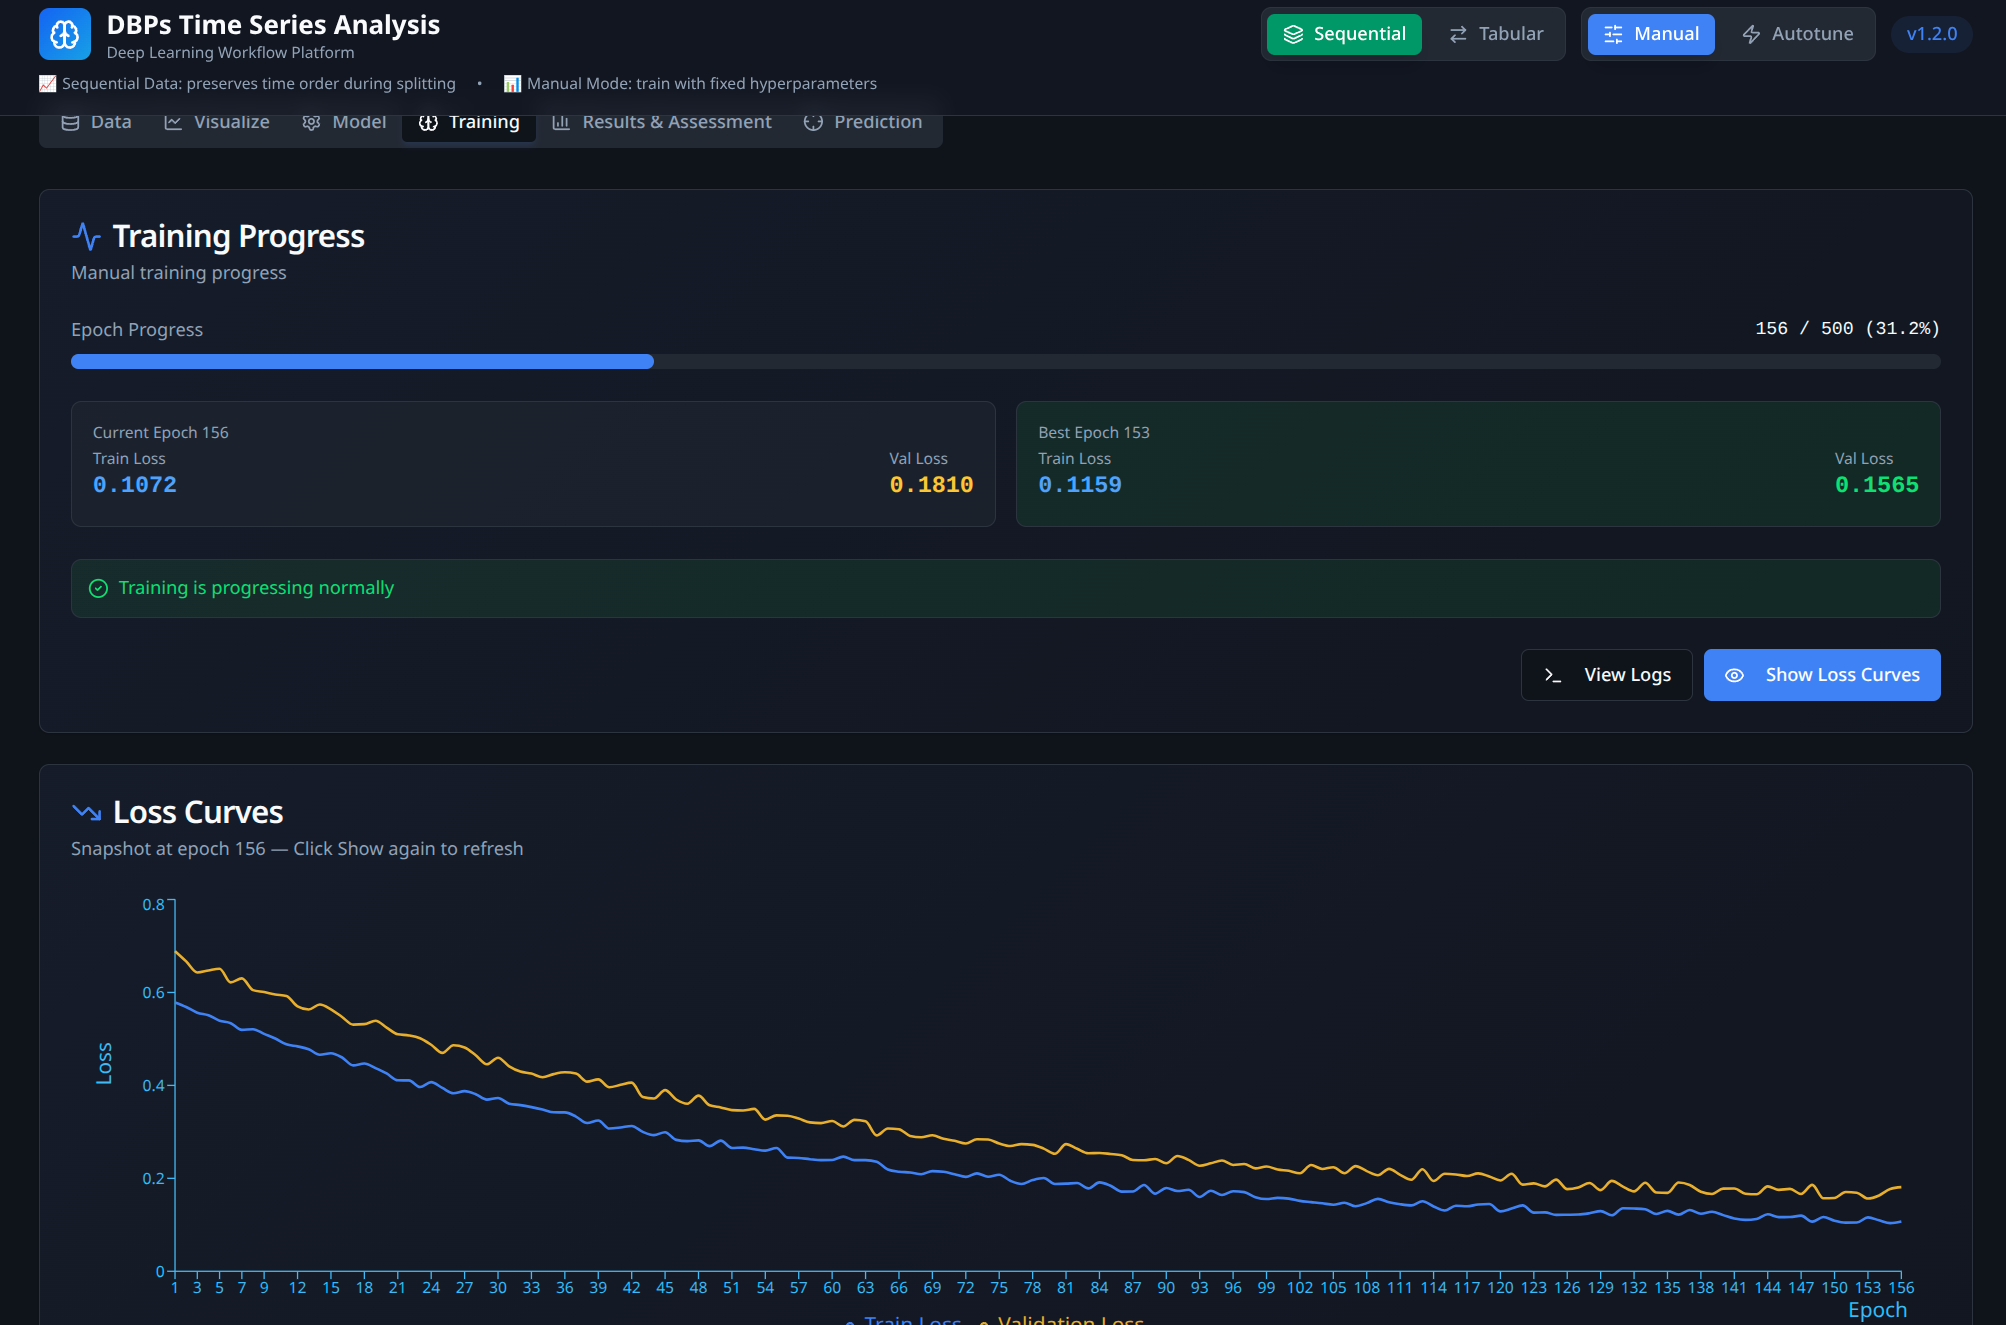
\includegraphics[width=\textwidth]{../attachment/frontend.png}
      \end{column}
  \end{columns}
\end{frame}

\subsection{Live Demo}
\begin{frame}
  \centering
  \Huge \textbf{Live Demonstration} \\
  \vspace{1cm}
  \Large (1:30 Video Walkthrough of the GUI Application)
  \vspace{1cm}
  \normalsize \\ Please direct your attention to the video player.
\end{frame}

% ============================================================================
% Section 4: Results & Conclusion
% ============================================================================
\section{Results \& Conclusion}

\subsection{Results}
\begin{frame}{Evaluation Environment \& GBDT Metrics}
  \begin{block}{Hardware}
    Environment: Fedora 43, NVIDIA RTX 4070 GPU.
  \end{block}
  
  \begin{table}
      \centering
      \caption{Overall Performance Metrics for GBDT Models (CAWW\_29)}
      \begin{tabular}{lccc}
      \toprule
      \textbf{Model} & \textbf{MSE} & \textbf{MAE} & \textbf{RMSE} \\
      \midrule
      \textbf{XGBoost} & \textbf{0.2217} & \textbf{0.1920} & \textbf{0.4709} \\
      LightGBM & 0.8666 & 0.4017 & 0.9309 \\
      CatBoost & 2.0576 & 0.6288 & 1.4344 \\
      \bottomrule
      \end{tabular}
  \end{table}
  \small
  \textit{Note}: XGBoost outperforms others, but GBDTs lack natural representation learning for temporal data and extrapolate poorly.
\end{frame}

\begin{frame}{GBDT Models: Visualization (TRC-PPL2)}
  \begin{figure}
      \centering
      \resizebox{\textwidth}{!}{
      \begin{tabular}{ccc}
          \textbf{XGBoost} & \textbf{LightGBM} & \textbf{CatBoost} \\
          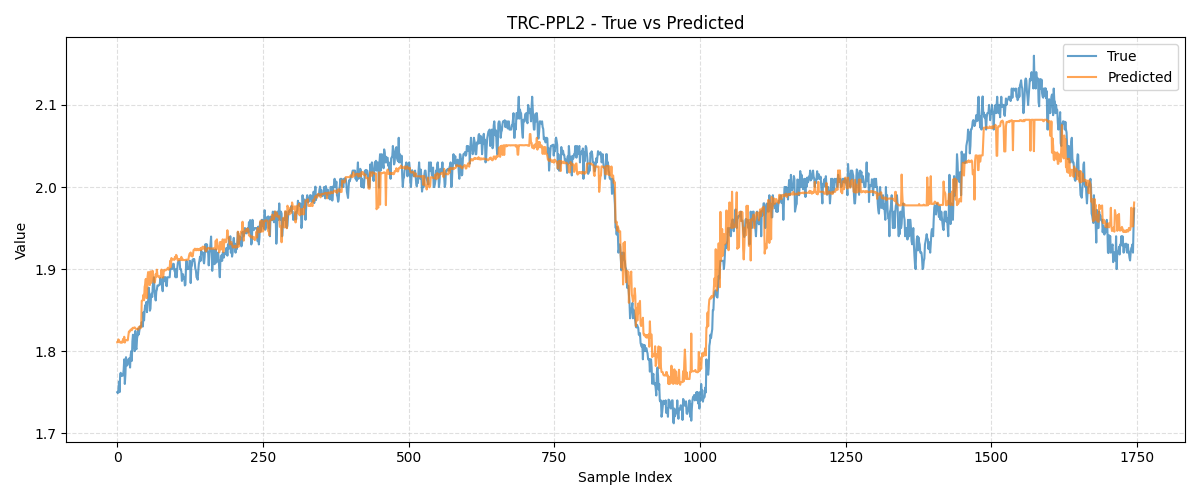
\includegraphics[width=0.33\linewidth]{../../Archived/final-results/caww29-results/xgboost/test_results/TRC-PPL2_pred_vs_true.png} &
          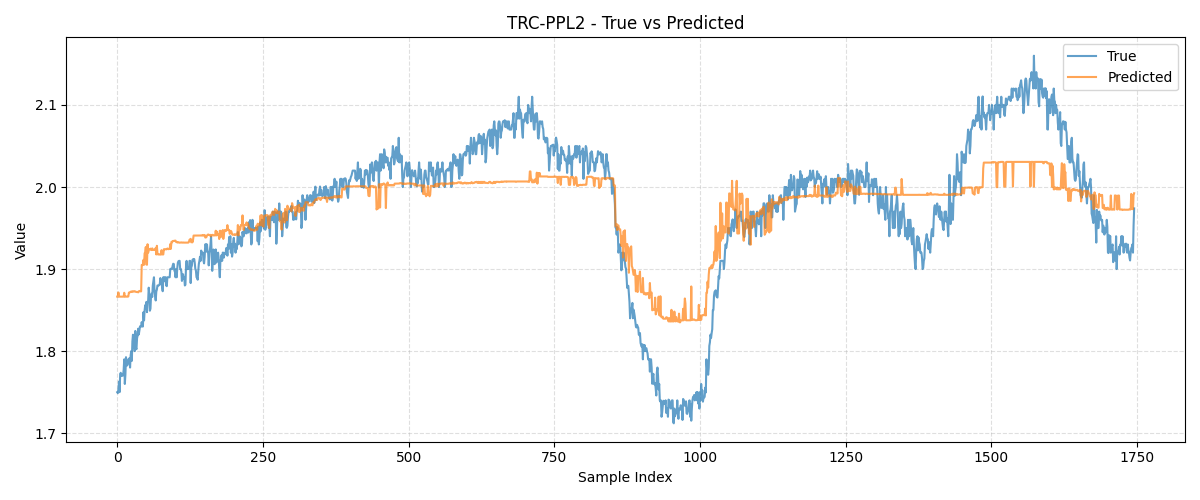
\includegraphics[width=0.33\linewidth]{../../Archived/final-results/caww29-results/lightgbm/test_results/TRC-PPL2_pred_vs_true.png} &
          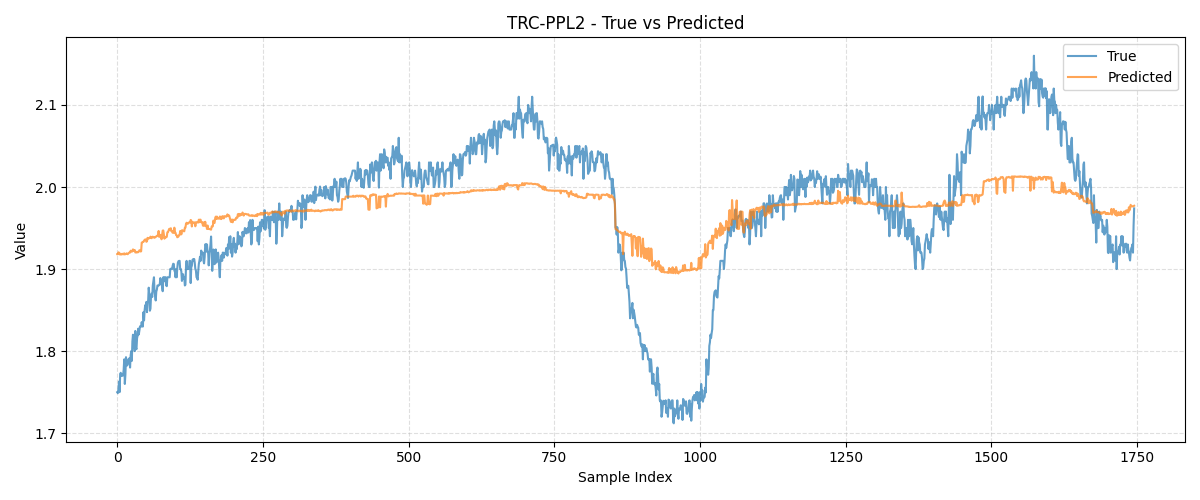
\includegraphics[width=0.33\linewidth]{../../Archived/final-results/caww29-results/catboost/test_results/TRC-PPL2_pred_vs_true.png} \\
          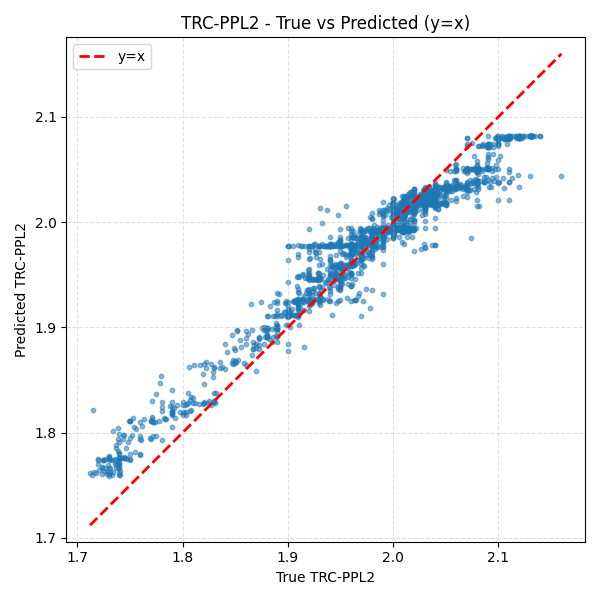
\includegraphics[width=0.33\linewidth]{../../Archived/final-results/caww29-results/xgboost/test_results/TRC-PPL2_yx_scatter.png} &
          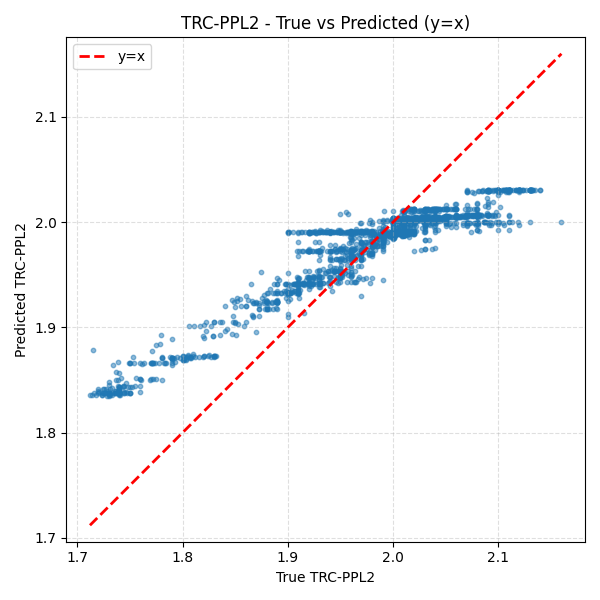
\includegraphics[width=0.33\linewidth]{../../Archived/final-results/caww29-results/lightgbm/test_results/TRC-PPL2_yx_scatter.png} &
          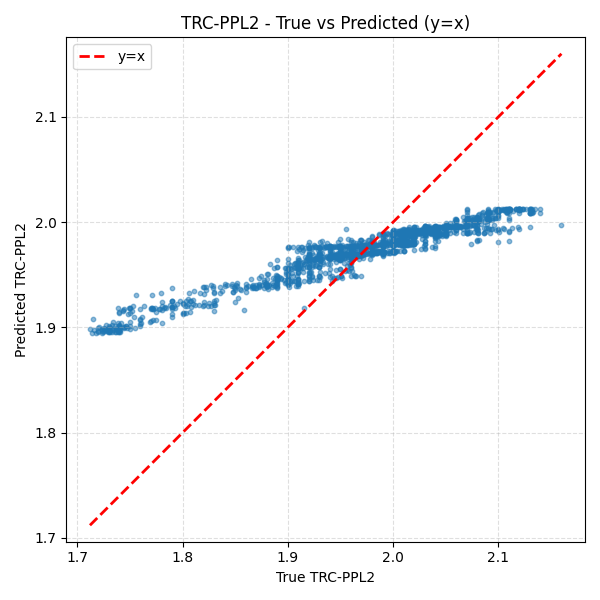
\includegraphics[width=0.33\linewidth]{../../Archived/final-results/caww29-results/catboost/test_results/TRC-PPL2_yx_scatter.png} \\
      \end{tabular}
      }
  \end{figure}
\end{frame}

\begin{frame}{Neural Network Metrics}
  \begin{table}
      \centering
      \caption{Overall Performance Metrics for Neural Network Models (CAWW\_29)}
      \begin{tabular}{lccc}
      \toprule
      \textbf{Model} & \textbf{MSE} & \textbf{MAE} & \textbf{RMSE} \\
      \midrule
      MLP & 0.2389 & 0.2046 & 0.4888 \\
      RNN & 0.4255 & 0.2678 & 0.6523 \\
      GRU & 0.2004 & 0.1921 & 0.4476 \\
      \textbf{LSTM} & \textbf{0.1779} & \textbf{0.1736} & \textbf{0.4218} \\
      Transformer & 0.4208 & 0.2789 & 0.6487 \\
      Mamba & 0.8168 & 0.3844 & 0.9038 \\
      \bottomrule
      \end{tabular}
  \end{table}
  \small
  \textit{Note}: LSTM achieves the lowest MSE on this specific dataset due to its gated mechanism being highly optimized for moderately long sequences.
\end{frame}

\begin{frame}{Neural Networks: Visualization (Part 1)}
  \begin{figure}
      \centering
      \resizebox{\textwidth}{!}{
      \begin{tabular}{ccc}
          \textbf{MLP} & \textbf{RNN} & \textbf{GRU} \\
          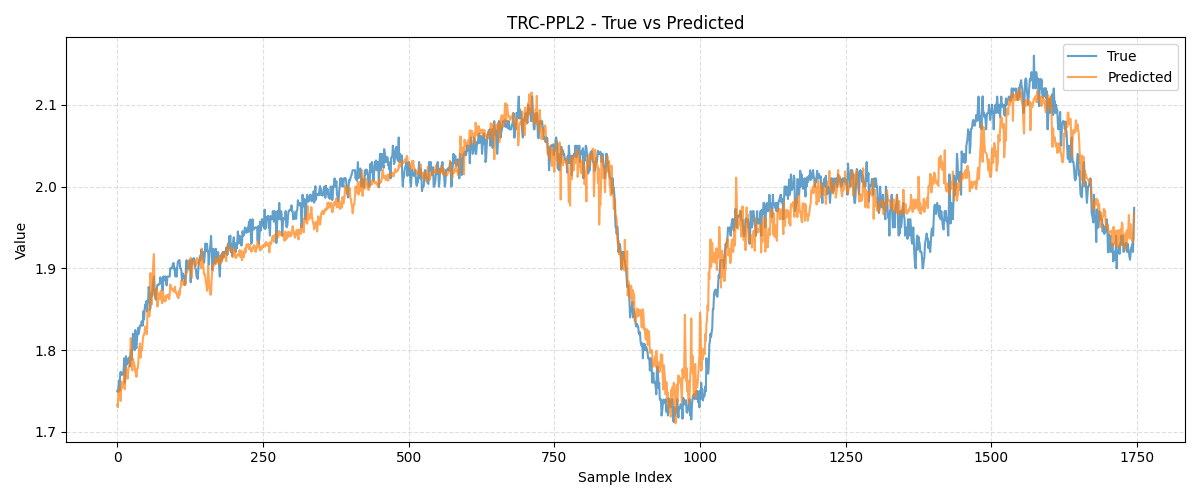
\includegraphics[width=0.33\linewidth]{../../Archived/final-results/caww29-results/mlp/test_results/TRC-PPL2_pred_vs_true.png} &
          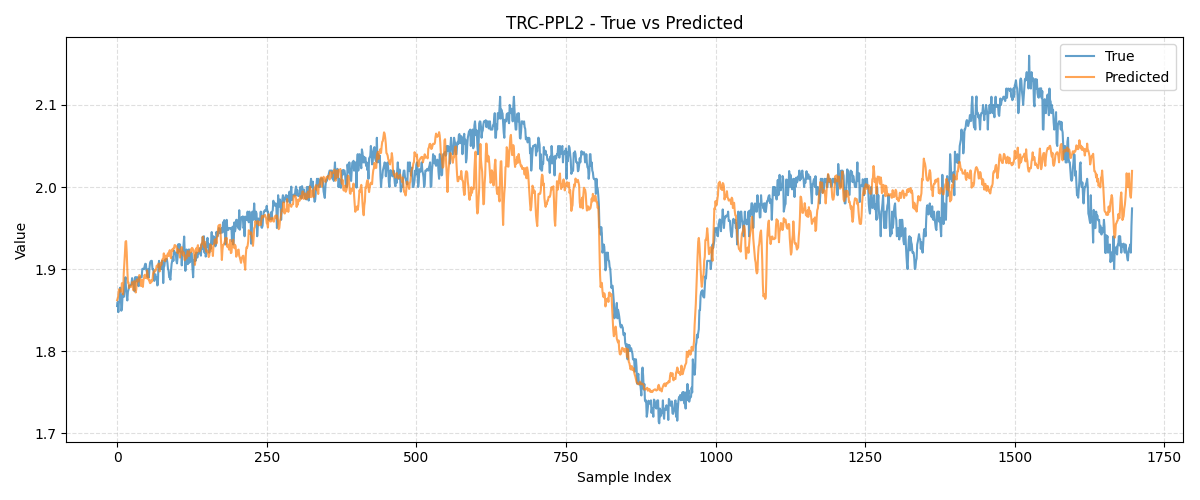
\includegraphics[width=0.33\linewidth]{../../Archived/final-results/caww29-results/rnn/test_results/TRC-PPL2_pred_vs_true.png} &
          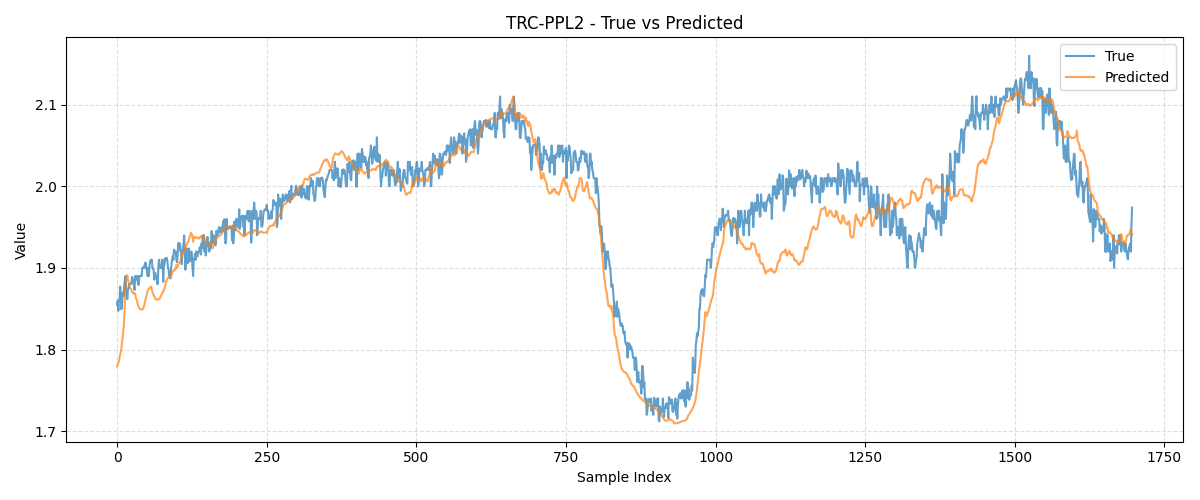
\includegraphics[width=0.33\linewidth]{../../Archived/final-results/caww29-results/gru/test_results/TRC-PPL2_pred_vs_true.png} \\
          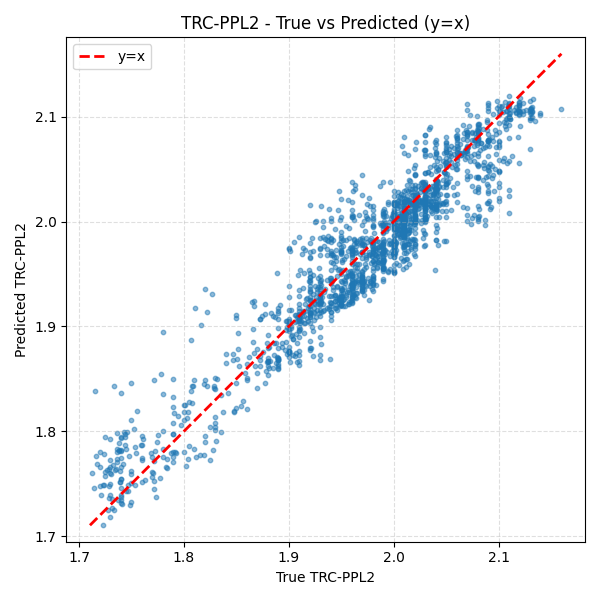
\includegraphics[width=0.33\linewidth]{../../Archived/final-results/caww29-results/mlp/test_results/TRC-PPL2_yx_scatter.png} &
          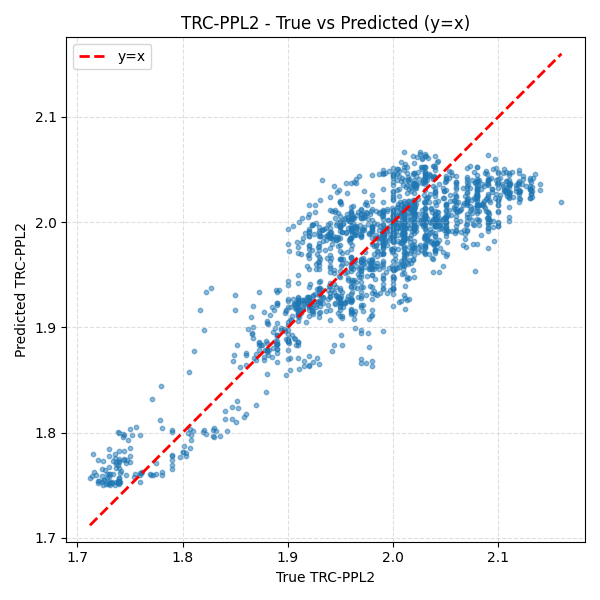
\includegraphics[width=0.33\linewidth]{../../Archived/final-results/caww29-results/rnn/test_results/TRC-PPL2_yx_scatter.png} &
          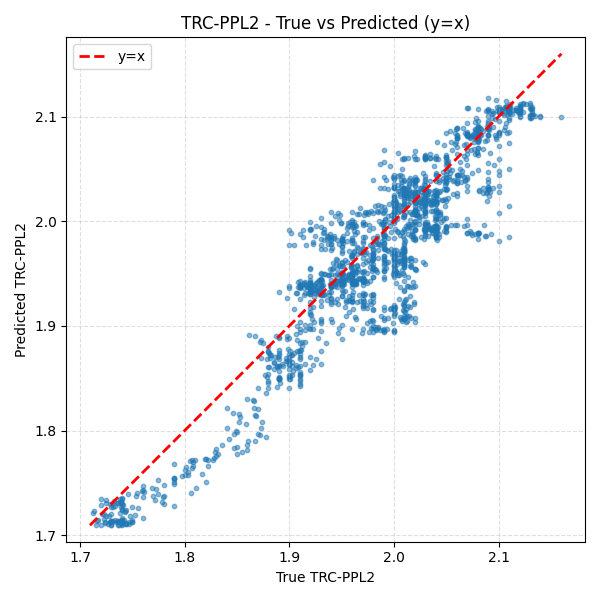
\includegraphics[width=0.33\linewidth]{../../Archived/final-results/caww29-results/gru/test_results/TRC-PPL2_yx_scatter.png} \\
      \end{tabular}
      }
  \end{figure}
\end{frame}

\begin{frame}{Neural Networks: Visualization (Part 2)}
  \begin{figure}
      \centering
      \resizebox{\textwidth}{!}{
      \begin{tabular}{ccc}
          \textbf{LSTM} & \textbf{Transformer} & \textbf{Mamba} \\
          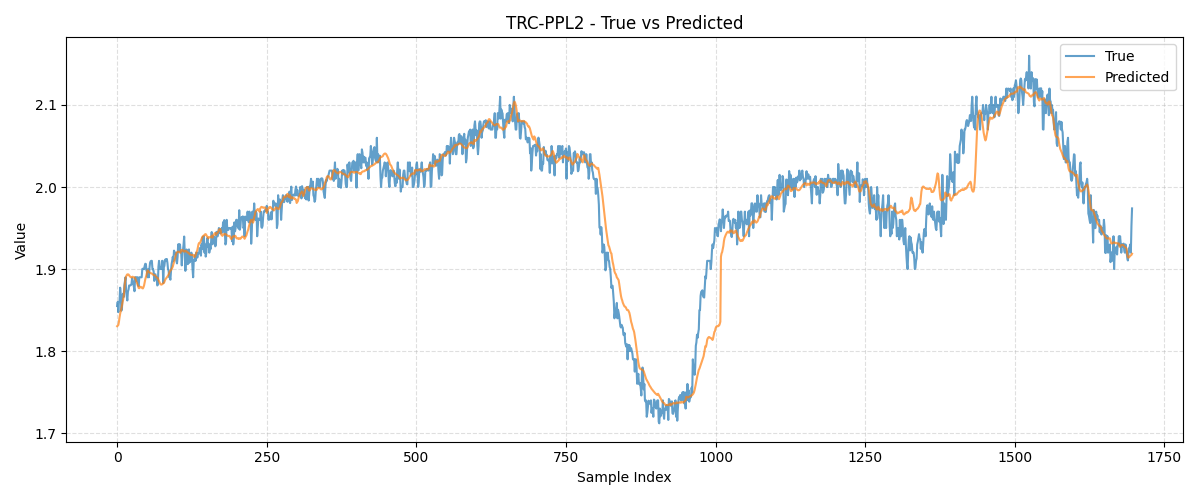
\includegraphics[width=0.33\linewidth]{../../Archived/final-results/caww29-results/lstm/test_results/TRC-PPL2_pred_vs_true.png} &
          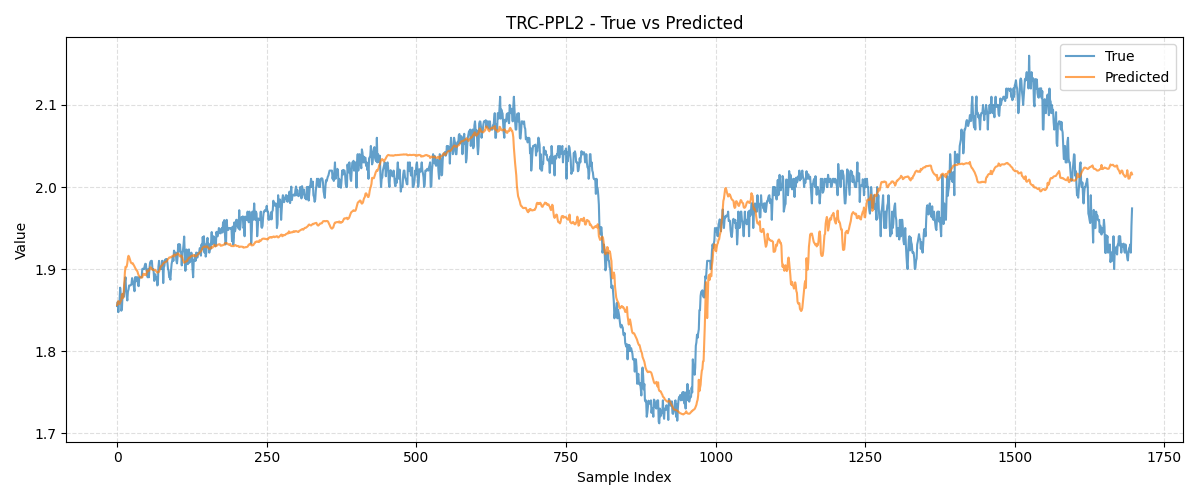
\includegraphics[width=0.33\linewidth]{../../Archived/final-results/caww29-results/transformer/test_results/TRC-PPL2_pred_vs_true.png} &
          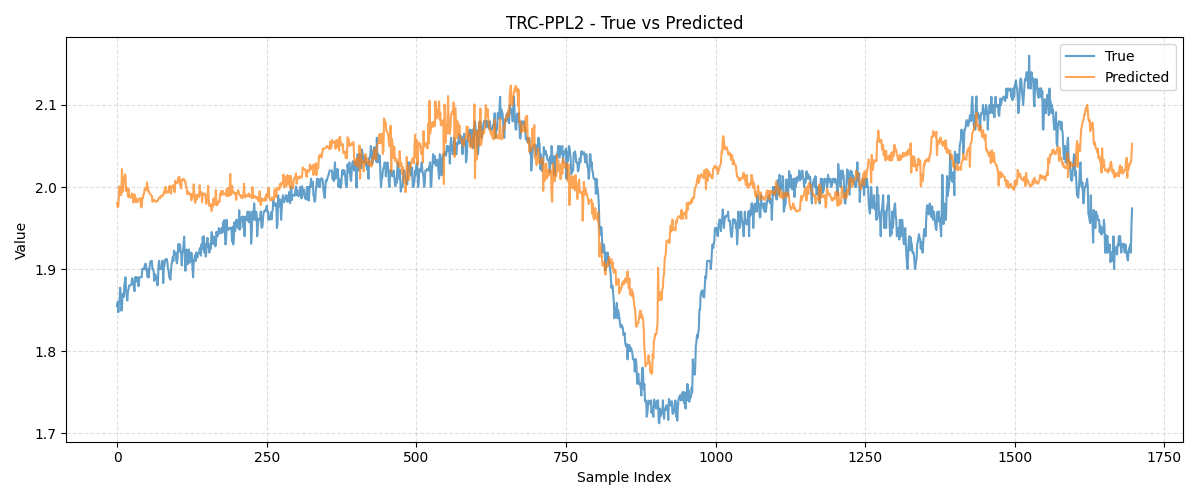
\includegraphics[width=0.33\linewidth]{../../Archived/final-results/caww29-results/mamba/test_results/TRC-PPL2_pred_vs_true.png} \\
          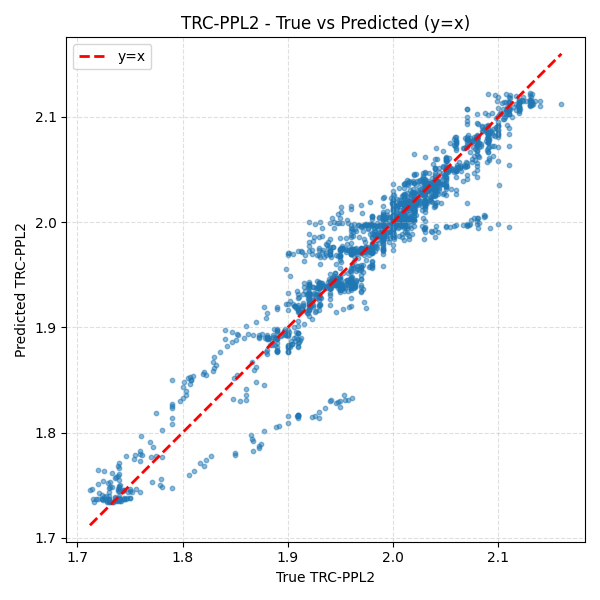
\includegraphics[width=0.33\linewidth]{../../Archived/final-results/caww29-results/lstm/test_results/TRC-PPL2_yx_scatter.png} &
          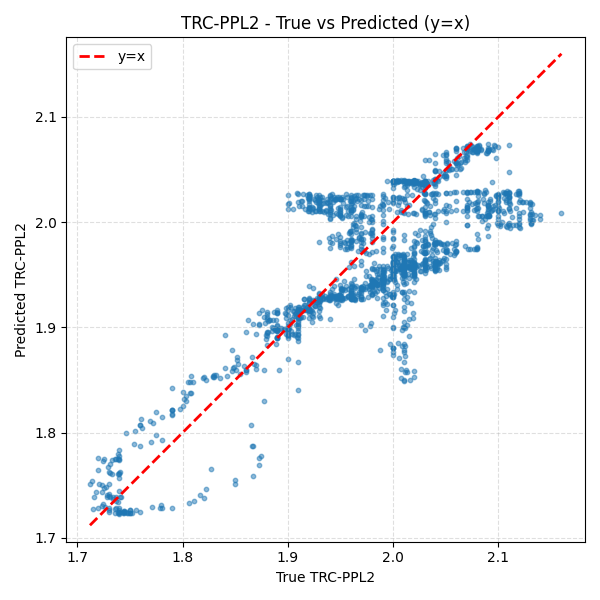
\includegraphics[width=0.33\linewidth]{../../Archived/final-results/caww29-results/transformer/test_results/TRC-PPL2_yx_scatter.png} &
          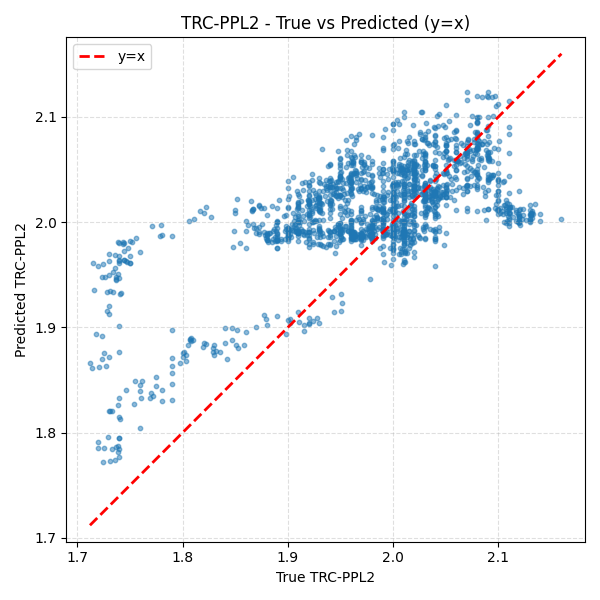
\includegraphics[width=0.33\linewidth]{../../Archived/final-results/caww29-results/mamba/test_results/TRC-PPL2_yx_scatter.png} \\
      \end{tabular}
      }
  \end{figure}
\end{frame}

\begin{frame}{Transformer Fine-Tuning Performance}
  \begin{table}
      \centering
      \caption{MSE of Fine-Tuning Strategies on $35^{\circ}\text{C}$ Datasets}
      \begin{tabular}{lcc}
      \toprule
      \textbf{Method} & \textbf{CAWW\_35 (MSE)} & \textbf{LSWW\_35 (MSE)} \\
      \midrule
      \textbf{Full Fine-Tuning} & \textbf{0.2624} & 0.8603 \\
      \textbf{Partial (Frozen Layers)} & 0.3635 & \textbf{0.3812} \\
      Adapter & 0.4066 & 0.8985 \\
      \bottomrule
      \end{tabular}
  \end{table}
  \begin{block}{Analysis}
      \begin{itemize}
          \item \textbf{Full Fine-Tuning}: Works best with clean data and aligned distributions (CAWW).
          \item \textbf{Partial Fine-Tuning}: Superior robustness and acts as a regularizer when dealing with severe source/noise distribution shifts (LSWW).
          \item \textbf{Adapter}: Bottleneck dimension restricts expression capacity for this specific regression task.
      \end{itemize}
  \end{block}
\end{frame}

\subsection{Conclusion}
\begin{frame}{Conclusion}
  \begin{block}{Key Takeaways}
      \begin{itemize}
          \item \textbf{Architecture Superiority}: LSTM yielded the highest baseline accuracy for continuous WDS time-series data.
          \item \textbf{Transfer Learning}: Transformer architectures demonstrated exceptionally strong generalization capabilities through Partial Fine-Tuning across distinct source distributions.
          \item \textbf{Industrial Readiness}: The developed GUI application successfully bridges advanced ML research with accessible industrial operation.
      \end{itemize}
  \end{block}
\end{frame}

\subsection{Future Work}
\begin{frame}{Future Work}
  \begin{block}{Next Steps}
      \begin{itemize}
          \item \textbf{Model Interpretability}: Integrate SHAP (SHapley Additive exPlanations) values to interpret exactly which sensor features drive the model's decisions temporally.
          \item \textbf{Second-Stage Model}: Map the accurately predicted proxy water quality parameters (TRC, TOC) directly to laboratory-measured actual THM and HAA concentrations.
      \end{itemize}
  \end{block}
\end{frame}

\begin{frame}{Conceptual Roadmap}
  \begin{figure}
      \centering
      \includegraphics[width=0.9\textwidth]{../attachment/experiment framework.png}
      \caption{Conceptual Roadmap for Future Integration}
  \end{figure}
\end{frame}

\begin{frame}
  \centering
  \Huge \textbf{Thank You!} \\
  \vspace{1cm}
  \Large Q \& A
\end{frame}

\end{document}
